\documentclass{beamer}
\usepackage[utf8]{inputenc}

\usetheme{Madrid}
\usecolortheme{default}
\usepackage{amsmath,amssymb,amsfonts,amsthm}
\usepackage{txfonts}
\usepackage{tkz-euclide}
\usepackage{listings}
\usepackage{adjustbox}
\usepackage{array}
\usepackage{tabularx}
\usepackage{gvv}
\usepackage{lmodern}
\usepackage{circuitikz}
\usepackage{tikz}
\usepackage{graphicx}

\setbeamertemplate{page number in head/foot}[totalframenumber]

\usepackage{tcolorbox}
\tcbuselibrary{minted,breakable,xparse,skins}



\definecolor{bg}{gray}{0.95}
\DeclareTCBListing{mintedbox}{O{}m!O{}}{%
	breakable=true,
	listing engine=minted,
	listing only,
	minted language=#2,
	minted style=default,
	minted options={%
		linenos,
		gobble=0,
		breaklines=true,
		breakafter=,,
		fontsize=\small,
		numbersep=8pt,
		#1},
	boxsep=0pt,
	left skip=0pt,
	right skip=0pt,
	left=25pt,
	right=0pt,
	top=3pt,
	bottom=3pt,
	arc=5pt,
	leftrule=0pt,
	rightrule=0pt,
	bottomrule=2pt,
	toprule=2pt,
	colback=bg,
	colframe=orange!70,
	enhanced,
	overlay={%
		\begin{tcbclipinterior}
			\fill[orange!20!white] (frame.south west) rectangle ([xshift=20pt]frame.north west);
	\end{tcbclipinterior}},
	#3,
}
\lstset{
	language=C,
	basicstyle=\ttfamily\small,
	keywordstyle=\color{blue},
	stringstyle=\color{orange},
	commentstyle=\color{green!60!black},
	numbers=left,
	numberstyle=\tiny\color{gray},
	breaklines=true,
	showstringspaces=false,
}
%------------------------------------------------------------
%This block of code defines the information to appear in the
%Title page
\title %optional
{7.4.43}
\date{}
%\subtitle{A short story}

\author % (optional)
{M Chanakya Srinivas- EE25BTECH11036}




\begin{document}


\frame{\titlepage}



% Slide 1: Problem
\begin{frame}{Problem Statement}
A circle passes through three points $A, B, C$ with $AC$ as its diameter.  
A line through $A$ intersects chord $BC$ at $D$.  

If $\angle DAB = \alpha$, $\angle CAB = \beta$, and the distance between $A$ and the midpoint of $DC$ is $d$, prove that the area of the circle is
\[
\frac{\pi d^2 \cos^2 \alpha}{\cos^2 \alpha + \cos^2 \beta + 2 \cos \alpha \cos \beta \cos(\beta - \alpha)}.
\]
\end{frame}

% Slide 2: Setup
\begin{frame}{Vector Setup}
Let
\[
\vec{A}, \vec{B}, \vec{C} \in \mathbb{R}^2
\]
be position vectors of $A,B,C$, with $AC$ as the diameter.  

The line through $A$ intersects $BC$ at $D$, and the midpoint of $DC$ is
\begin{align}
\vec{M} &= \frac{\vec{D} + \vec{C}}{2}, \\
d &= \|\vec{A} - \vec{M}\|.
\end{align}

Cosines of angles:
\begin{align}
\cos \alpha &= \frac{(\vec{B}-\vec{A})^T (\vec{D}-\vec{A})}{\|\vec{B}-\vec{A}\| \, \|\vec{D}-\vec{A}\|},\\
\cos \beta &= \frac{(\vec{C}-\vec{A})^T (\vec{B}-\vec{A})}{\|\vec{C}-\vec{A}\| \, \|\vec{B}-\vec{A}\|}.
\end{align}
\end{frame}

% Slide 3: Circle Radius
\begin{frame}{Circle Radius}
Since $AC$ is the diameter:
\begin{align}
r &= \frac{1}{2} \|\vec{A}-\vec{C}\|.
\end{align}

Let $D$ lie on chord $BC$ parametrically:
\begin{align}
\vec{D} &= \vec{B} + t (\vec{C}-\vec{B}), \quad 0 < t < 1.
\end{align}

Then midpoint $M$:
\begin{align}
\vec{M} &= \frac{\vec{D} + \vec{C}}{2} = \frac{1+t}{2}\vec{C} + \frac{1-t}{2}\vec{B}.
\end{align}

Vector from $A$ to $M$:
\begin{align}
\vec{M} - \vec{A} = \frac{1+t}{2}\vec{C} + \frac{1-t}{2}\vec{B} - \vec{A}.
\end{align}
\end{frame}

% Slide 4: Relation between r and d
\begin{frame}{Relation between $r$ and $d$}
The squared distance is
\begin{align}
d^2 &= \|\vec{M} - \vec{A} \|^2 = \left\| \frac{1+t}{2}\vec{C} + \frac{1-t}{2} \vec{B} - \vec{A} \right\|^2.
\end{align}

Solving for $\|\vec{A}-\vec{C}\|$ in terms of $d$, $\alpha$, $\beta$:
\begin{align}
\|\vec{A}-\vec{C}\|^2 
= \frac{4 d^2 \cos^2 \alpha}{\cos^2 \alpha + \cos^2 \beta + 2 \cos \alpha \cos \beta \cos(\beta - \alpha)}.
\end{align}

Radius squared:
\begin{align}
r^2 &= \frac{1}{4}\|\vec{A}-\vec{C}\|^2 
= \frac{d^2 \cos^2 \alpha}{\cos^2 \alpha + \cos^2 \beta + 2 \cos \alpha \cos \beta \cos(\beta-\alpha)}.
\end{align}
\end{frame}

% Slide 5: Area of Circle
\begin{frame}{Area of Circle}
\begin{align}
\text{Area} &= \pi r^2 \\
&= \frac{\pi d^2 \cos^2 \alpha}{\cos^2 \alpha + \cos^2 \beta + 2 \cos \alpha \cos \beta \cos(\beta-\alpha)}.
\end{align}

\begin{center}
\boxed{\text{Area of circle } = \frac{\pi d^2 \cos^2 \alpha}{\cos^2 \alpha + \cos^2 \beta + 2 \cos \alpha \cos \beta \cos(\beta - \alpha)}}
\end{center}
\end{frame}





\begin{frame}[fragile]{C Code}
\begin{lstlisting}
#include <stdio.h>
#include <math.h>

typedef struct {
    double x, y;
} Vec;

// Vector subtraction
Vec sub(Vec a, Vec b) {
    Vec r = {a.x - b.x, a.y - b.y};
    return r;
}

// Midpoint
Vec midpoint(Vec a, Vec b) {
    Vec r = {(a.x + b.x)/2.0, (a.y + b.y)/2.0};
    return r;
}

 \end{lstlisting}
\end{frame}
\begin{frame}[fragile]{C Code}
\begin{lstlisting}
// Dot product
double dot(Vec a, Vec b) {
    return a.x*b.x + a.y*b.y;
}

// Norm
double norm(Vec a) {
    return sqrt(dot(a,a));
}

// Circle center (midpoint of AC)
Vec circle_center(Vec A, Vec C) {
    return midpoint(A, C);
}

// Midpoint of DC
Vec midpoint_DC(Vec D, Vec C) {
    return midpoint(D, C);
}

 \end{lstlisting}
\end{frame}
\begin{frame}[fragile]{Python code through shared output}
\begin{lstlisting}
import ctypes
import numpy as np
import matplotlib.pyplot as plt
from matplotlib.patches import Arc

# Load shared library
lib = ctypes.CDLL("./libgeom.so")

class Vec(ctypes.Structure):
    _fields_ = [("x", ctypes.c_double), ("y", ctypes.c_double)]

# Bind functions
lib.circle_center.argtypes = [Vec, Vec]
lib.circle_center.restype = Vec

lib.midpoint_DC.argtypes = [Vec, Vec]
lib.midpoint_DC.restype = Vec

# Shift circle upward for clarity
A = Vec(0,1)
C = Vec(2,1)
B = Vec(1,2)
D = Vec(1.5,1.5)
 \end{lstlisting}
\end{frame}
\begin{frame}[fragile]{Python code through shared output}
\begin{lstlisting}
O = lib.circle_center(A,C)
M = lib.midpoint_DC(D,C)

# Convert to numpy
def vec2np(v): return np.array([v.x, v.y])
An,Bn,Cn,Dn,On,Mn = map(vec2np,[A,B,C,D,O,M])

# Circle
r = np.linalg.norm(Cn - An)/2
theta = np.linspace(0,2*np.pi,400)
circle_x = On[0] + r*np.cos(theta)
circle_y = On[1] + r*np.sin(theta)

fig, ax = plt.subplots(figsize=(6,6))
ax.plot(circle_x, circle_y, 'b')

# Points
for P,name in zip([An,Bn,Cn,Dn,Mn,On],['A','B','C','D','M','O']):
    ax.plot(P[0],P[1],'ro')
    ax.text(P[0]+0.05,P[1]+0.05,name,fontsize=12)
 \end{lstlisting}
\end{frame}
\begin{frame}[fragile]{Python code through shared output}
\begin{lstlisting}
# Lines
ax.plot([Bn[0],Cn[0]],[Bn[1],Cn[1]],'g--',label="$BC$")
ax.plot([An[0],Dn[0]],[An[1],Dn[1]],'m--',label="$AD$")
ax.plot([An[0],Cn[0]],[An[1],Cn[1]],'k-', label="$AC$")
ax.plot([An[0],Bn[0]],[An[1],Bn[1]],'c-', label="$AB$")  # New AB

# Function to draw arcs for angles
def draw_angle(ax, center, p1, p2, radius=0.25, label=""):
    ang1 = np.degrees(np.arctan2(p1[1]-center[1], p1[0]-center[0]))
    ang2 = np.degrees(np.arctan2(p2[1]-center[1], p2[0]-center[0]))
    arc = Arc(center, 2*radius, 2*radius, angle=0,
              theta1=min(ang1,ang2), theta2=max(ang1,ang2),
    \end{lstlisting}
\end{frame}
\begin{frame}[fragile]{Python code through shared output}
\begin{lstlisting}
              color='k')
    ax.add_patch(arc)
    mid = (ang1+ang2)/2
    ax.text(center[0]+radius*np.cos(np.radians(mid)),
            center[1]+radius*np.sin(np.radians(mid)),
            label, fontsize=14, color="red")

# Angles at A
draw_angle(ax, An, Dn, Bn, radius=0.3, label=r"$\alpha$")
draw_angle(ax, An, Cn, Bn, radius=0.5, label=r"$\beta$")

# Aesthetics
ax.set_aspect(1)
ax.set_xlim(-0.5,2.5)
ax.set_ylim(0,2.5)
ax.legend(fontsize=10, loc="upper right")
plt.show()

 \end{lstlisting}
\end{frame}
\begin{frame}[fragile]{Only Python code}
\begin{lstlisting}
import numpy as np
import matplotlib.pyplot as plt
from numpy import linalg as LA
from conics.funcs import circ_gen
from line.funcs import line_gen
from matplotlib.patches import Arc

# === Step 1: Circle with diameter AC ===
A = np.array([0.0,0.0]).reshape(-1,1)
C = np.array([4.0,0.0]).reshape(-1,1)
O = (A + C)/2
R = LA.norm(C - O)

# === Step 2: Choose B on circle (not collinear with AC) ===
theta = np.deg2rad(60)
B = O + R * np.array([[np.cos(theta)], [np.sin(theta)]])
 \end{lstlisting}
\end{frame}
\begin{frame}[fragile]{Only Python code}
\begin{lstlisting}
# === Step 3: Angle alpha at A ===
alpha = np.deg2rad(30)  # angle DAB
slope_AD = np.tan(alpha)

# === Step 4: Compute intersection D on BC segment ===
dx = C[0,0] - B[0,0]
dy = C[1,0] - B[1,0]
t = (slope_AD*(A[0,0]-B[0,0]) + (B[1,0]-A[1,0])) / (dy - slope_AD*dx)
t = np.clip(t, 0.15, 0.85)  # ensure D inside BC
D = (B + t*(C-B)).reshape(-1,1)

# === Step 5: Midpoint M of DC ===
M = (D + C)/2

# === Step 6: Compute distance d = AM ===
d = LA.norm(A - M)
 \end{lstlisting}
\end{frame}
\begin{frame}[fragile]{Only Python code}
\begin{lstlisting}
# === Step 7: Generate circle and lines using your functions ===
x_circ = circ_gen(O,R)
x_AB = line_gen(A,B)
x_AC = line_gen(A,C)
x_BC = line_gen(B,C)
x_AD = line_gen(A,D)
x_DM = line_gen(D,M)

# === Step 8: Plot setup ===
plt.figure(figsize=(8,8))
plt.plot(x_circ[0,:], x_circ[1,:], 'b', lw=2, label='Circle')
plt.plot(x_AB[0,:], x_AB[1,:], 'g', label='AB')
plt.plot(x_AC[0,:], x_AC[1,:], 'k', label='AC (diameter)')
plt.plot(x_BC[0,:], x_BC[1,:], 'c', lw=2, label='BC (chord)')
plt.plot(x_AD[0,:], x_AD[1,:], 'r', lw=2, label='AD')
plt.plot(x_DM[0,:], x_DM[1,:], 'm--', lw=2, label='DC midpoint line')
 \end{lstlisting}
\end{frame}
\begin{frame}[fragile]{Only Python code}
\begin{lstlisting}
# === Step 9: Plot points ===
points = {'A':A,'B':B,'C':C,'D':D,'M':M,'O':O}
for name,p in points.items():
    plt.scatter(p[0,0], p[1,0], s=70, zorder=5)
    offset = 0.15
    if name in ['D','B','M']:
        offset = 0.25
    plt.text(p[0,0]+offset, p[1,0]+offset, name, fontsize=12, fontweight='bold')

# === Step 10: Draw angles alpha (DAB) and beta (CAB) clearly ===
def plot_angle(center, p1, p2, radius, color, label):
    v1, v2 = p1-center, p2-center
    ang1 = np.degrees(np.arctan2(v1[1,0], v1[0,0]))
    ang2 = np.degrees(np.arctan2(v2[1,0], v2[0,0]))
    if ang2 < ang1: ang1, ang2 = ang2, ang1
    arc = Arc((center[0,0], center[1,0]), 2*radius, 2*radius,
              angle=0, theta1=ang1, theta2=ang2, color=color, lw=3)
               \end{lstlisting}
\end{frame}
\begin{frame}[fragile]{Only Python code}
\begin{lstlisting}
    plt.gca().add_patch(arc)
    mid = np.radians((ang1+ang2)/2)
    plt.text(center[0,0]+1.4*radius*np.cos(mid),
             center[1,0]+1.4*radius*np.sin(mid),
             label, fontsize=16, color=color, fontweight='bold')

plot_angle(A,D,B,0.5,'r',r'$\alpha$')  # DAB
plot_angle(A,C,B,0.8,'b',r'$\beta$')   # CAB
 \end{lstlisting}
\end{frame}
\begin{frame}[fragile]{Only Python code}
\begin{lstlisting}
# === Step 11: Annotate distance d = AM ===
plt.plot([A[0,0], M[0,0]], [A[1,0], M[1,0]], 'k--', lw=1.5)
mid_label = (A + M)/2
plt.text(mid_label[0,0], mid_label[1,0]+0.15, f'd={d:.2f}', fontsize=12, fontweight='bold', color='k')

# === Step 12: Finalize plot ===
plt.axis('equal')
plt.grid(True)
plt.legend(fontsize=12)
plt.title('Circle with AC as diameter, D on BC, midpoint M, angles α and β, distance d', fontsize=14)
plt.show()

 \end{lstlisting}
\end{frame}
\begin{frame}{PLOTS}
    \begin{figure}
        \centering
        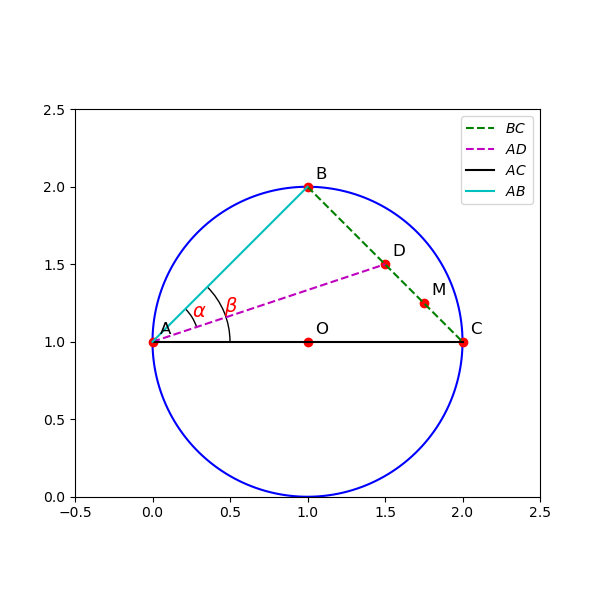
\includegraphics[width=0.75\columnwidth]{figs/fig1.png}
        \caption{}
        \label{fig:placeholder}
    \end{figure}
\end{frame}
\begin{frame}{PLOTS}
   \begin{figure}
        \centering
        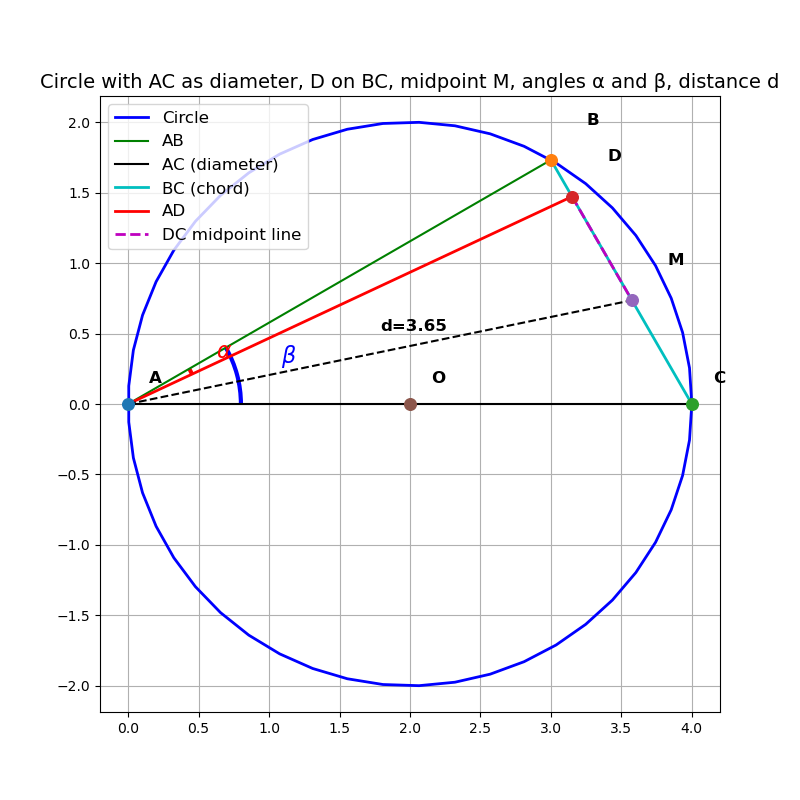
\includegraphics[width=0.75\columnwidth]{figs/fig2.png}
        \caption{}
        \label{fig:placeholder}
    \end{figure} 
\end{frame}
\end{document}
